%
%
%
\section{Potentials}

\subsection{The effective potential}

Fundamental to the electronic structure problem in density functional theory is solving the set of one-electron Kohn-Sham equations, as give by

\begin{equation}
    \left(-\frac{1}{2}\nabla^{2} + \nu_{\text{eff}}\right)\varphi(\vec{r}) = \epsilon \varphi(\vec{r})
\end{equation}

where $\epsilon$ is the one-electron energy and $\nu_{\text{eff}}$ the effective potential which is composed out of three parts. These three parts are given by

\begin{equation}
    \nu_{\text{eff}}(\vec{r}) = \nu_{\text{ext}}(\vec{r}) + \nu_{u}(\vec{r}) + \nu_{\text{xc}}(\vec{r})
\end{equation}

where $\nu_{\text{ext}}$ is the attractive field due to the set of nuclei, $\nu_{u}(\vec{r})$ is the classical coulombic potential, termed the Hartree potential, and $\nu_{\text{xc}}$ the exchange-correlation potential, encapsulating electron-exchange and -correlation effects.

The external potential $\nu_{\text{ext}}$ depends solely on the position of the nuclei whereas the Hartree and exchange-correlation potentials depend on the electron density $\rho(\vec{r})$. These three potentials can be represented both in real-space, or by their reciprocal-space counterparts indicated by $\tilde{\nu}_{\text{ext}}(\vec{G})$, $\tilde{\nu}_{u}(\vec{G})$ and $\tilde{\nu}_{\text{xc}}(\vec{G})$. It turns out that the external and Hartree potential can be rather easily constructed in reciprocal-space, whereas the exchange-correlation functional is best constructed in real-space. Here, we will show how this is achieved.

%
%
%
\subsection{Poisson's equation}

Given a charge density function $\rho(\vec{r})$, the electrostatic potential can be readily calculated by solving Poisson's equation\footnote{Note that I here already assume that $\rho(\vec{r})$ corresponds to a negative charge density. If $\rho(\vec{r})$ pertains to a positive charge density, there would be no minus sign on the right-hand side of this equation.}

\begin{equation}
    \nabla^{2} \varphi (\vec{r}) = -4\pi\rho(\vec{r}).
    \label{eq:poisson}
\end{equation}

Suppose that we expand the charge density as a set of plane waves, as shown earlier, such that

\begin{equation}
    \rho(\vec{r}) = \frac{1}{\sqrt{\Omega}} \sum_{\vec{G}} \tilde{\rho}(\vec{G}) \exp \left(i \vec{G} \cdot \vec{r} \right).
    \label{eq:charge_expansion}
\end{equation}

Insertion of \cref{eq:charge_expansion} into \cref{eq:poisson} provides the following second-order differential equation

\begin{equation}
    \nabla^{2} \varphi (\vec{r}) = -\frac{4\pi}{\sqrt{\Omega}} \sum_{\vec{G}} \nabla^{2} \tilde{\rho}(\vec{G}) \exp \left(i \vec{G} \cdot \vec{r} \right).
\end{equation}

which can be readily solved, yielding

\begin{equation}
    \varphi (\vec{r}) = -\frac{4\pi}{\sqrt{\Omega}} \sum_{\vec{G}} \frac{\tilde{\rho}(\vec{G})}{|\vec{G}|^{2}} \exp \left(i \vec{G} \cdot \vec{r} \right).
\end{equation}

The observant reader has most likely identified the problematic term $\vec{G} = \vec{0}$, which produces a singularity. This term is therefore neglected and effectively the following equation is used.

\begin{equation}
    \varphi (\vec{r}) = -\frac{4\pi}{\sqrt{\Omega}} \sum_{\vec{G} \neq \vec{0}} \frac{\tilde{\rho}(\vec{G})}{|\vec{G}|^{2}} \exp \left(i \vec{G} \cdot \vec{r} \right).
\end{equation}

The above expression is equivalent to

\begin{equation}
    \varphi (\vec{r}) = \mathcal{F}_{\text{pw}}^{-1} \left[-\frac{4 \pi}{|\vec{G}|^{2}} \mathcal{F}_{\text{pw}} \left[\rho(\vec{r}) \right] \right]_{\vec{G} \neq \vec{0}}.
    \label{eq:hartree-pot}
\end{equation}

In other words, the external and Hartree potential can be readily obtained via the following recipe\footnote{For the external potential, generated by a set of positive point charges, \cref{eq:poisson} would not have the negative sign.} 

\begin{enumerate}
    \item Perform a FFT on the charge density.
    \item Modify the coefficient and set $\tilde{\rho}(\vec{G} = \vec{0}) = 0$.
    \item Perform an inverse FFT to obtain the electrostatic potential.
\end{enumerate}

From the above derivation it can also be observed that the type of normalization constant used in the plane wave expansion is arbitrary as always a combination of a forward and backward (inverse) Fourier transform occurs. Thus, if one uses $\mathcal{F}$ and $\mathcal{F}^{-1}$ in \cref{eq:hartree-pot}, the same result will be found.

%
%
%
\subsection{The external potential}

The external potential is generated by the nuclei in the unit cell. Point charges are represented by the Dirac delta function, such that the charge density of the nuclei is given by

\begin{equation}
    \rho_{\text{nuclii}}(\vec{r}) = \sum_{j} q_{j} \delta(\vec{r} - \vec{R_{j}}).
\end{equation}

Performing the FFT over a set of point charges is due to the discrete nature of the algorithm rather difficult. Perhaps more importantly, direct application of \cref{eq:pwcoeff-int} is actually very straightforward for a Dirac delta function and gives

\begin{align}
    \braket{\phi(\vec{G},\vec{r}) | u(\vec{r})} &= \frac{1}{\sqrt{\Omega}} \int_{\Omega} d\vec{r} \; \sum_{\vec{G}} \exp \left(i\vec{G} \cdot \vec{r} \right) \cdot \delta(\vec{r} - \vec{R_{j}}) \\
    &= \frac{1}{\sqrt{\Omega}} \exp \left(i \vec{G} \cdot \vec{R}_{j} \right).
\end{align}

Generalizing this results, we find

\begin{equation}
    \mathcal{F}_{\text{pw}} \left[\sum_{j} q_{j} \delta(\vec{r} - \vec{R_{j}})\right] = \frac{1}{\sqrt{\Omega}} \sum_{\vec{G}} \sum_{j} \exp \left(i \vec{G} \cdot \vec{R}_{j} \right).
\end{equation}

Thus, the nuclear attraction potential can be found via

\begin{equation}
    \nu_{\text{ext}} = -\frac{4 \pi}{\sqrt{\Omega}} \mathcal{F}_{\text{pw}}^{-1} \left[\sum_{_{\vec{G} \neq \vec{0}}} |\vec{G}|^{-2} \sum_{j} \exp \left(i \vec{G} \cdot \vec{R}_{j} \right) \right].
    \label{eq:nucpotpw}
\end{equation}

%
%
%
\subsubsection{Demonstration for the 1s orbital of H}

To demonstrate the above theory, let us revisit the toy problem of a hydrogen atom. For this atom, the electronic potential energy can be calculated analytically and corresponds to

\begin{align}
    E_{\text{pot}} &= \left<\psi_{1s} \left| \frac{1}{r} \right| \psi_{1s}\right> \\
    &= 4 \pi \int dr \; r^{2} \; \cdot \left(\frac{1}{r}\right) \cdot |\psi_{1s}|^{2} \\
    &= 4 \pi \int dr \; r \; \exp \left(-2r \right) \\
    &= -1.
\end{align}

For a single hydrogen atom, \cref{eq:nucpotpw} reduces to

\begin{equation}
    \nu_{\text{ext}} = -\frac{4 \pi}{\sqrt{\Omega}} \mathcal{F}_{\text{pw}}^{-1} \left[ \sum_{\vec{G} \neq \vec{0}} |\vec{G}|^{-2} \exp \left(i \vec{G} \cdot \vec{R} \right) \right]
    \label{eq:nucpotpw}
\end{equation}

and we can approximate $E_{\text{pot}}$ by means of the following numerical integration

\begin{equation}
    E_{\text{pot}} = \frac{\Omega}{N} \sum_{i}^{N} \nu_{\text{ext}}(\vec{r}_{i}) |\psi_{1s}(\vec{r}_{i})|^{2}.
    \label{eq:nucpotpw}
\end{equation}

where $N$ represents the number of sampling points and $\frac{\Omega}{N}$ is the volume corresponding to such a sampling point.

In \cref{fig:nuclear_attraction}, the electronic potential energy as function of the cubic unit cell edge size $a_{0}$ and the number of sampling points per Cartesian direction is shown. From this Figure, it is clear that in the limit of a very large number of plane waves (sampling points), we approach the analytical solution of -1.0 Ht.

\begin{Figure}
    \centering
    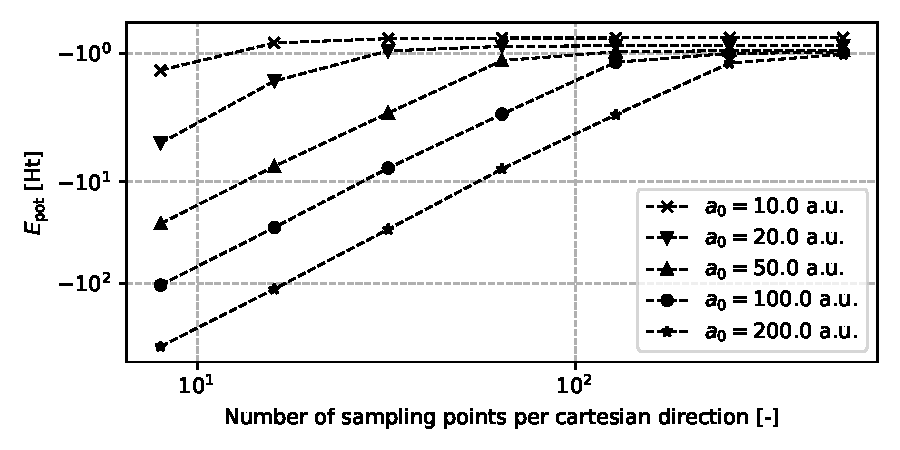
\includegraphics[width=\linewidth]{img/nuclear_attraction.pdf}
    \captionof{figure}{Potential energy of a hydrogen atom as function of the number of plane waves and the dimension of the unit cell.}
    \label{fig:nuclear_attraction}
\end{Figure}

Nevertheless, a proper match with the analytical result is absent, especially for smaller unit cell sizes. This relatively large discrepancy is caused by the omission of the divergent $\vec{G}=\vec{0}$ term, whose influence is larger for smaller unit cells. For the calculation of the Hartree potential and the Ewald sum (\textit{vide infra}), similar divergent terms appear and these terms tend to cancel each other out. This implies that one cannot readily use the result of a single component of the calculation, but one has to combine all the electrostatic contributions and only then a valid comparison with an analytical solution can be made.

%
%
%
\subsection{The Hartree potential}

\cref{eq:hartree-pot} can be readily used to calculate the Hartree potential from a charge density distribution. We should however be wary of the fact that we have removed the divergent term corresponding to $\vec{G} = \vec{0}$. To understand the consequence of that, let us here apply \cref{eq:hartree-pot} to a normalized wave function corresponding to a Gaussian, i.e.

\begin{equation}
    \phi(\vec{r}) = \left(\frac{2}{\pi} \right)^{3/4} \exp \left(-|\vec{r}|^{2} \right).
\end{equation}

The electrostatic energy due to the repelling electrons constituting the density, i.e. $\rho = |\phi(\vec{r})|^{2}$, can be calculated analytically\footnote{Its derivation is beyond the scope of this work, but can be found in ``Modern Quantum Chemistry'' of Szabo and Ostlund. It corresponds to equation A.41 in that book wherein you use $\alpha=\beta=\gamma=\delta=0$ and $\vec{R}_{A}=\vec{R}_{B}=\vec{R}_{C}=\vec{R}_{D}=0$.} and corresponds to

\begin{equation}
    E_{\text{e-e}} = \left<\phi(\vec{r}_{1})\phi(\vec{r}_{2})\left|\frac{1}{r_{12}}\right|\phi(\vec{r}_{1})\phi(\vec{r}_{2})\right> = \frac{2}{\sqrt{\pi}}.
\end{equation}

In the top graph of \cref{fig:electrostatics}, the energy corresponding to the electron-electron repulsion $E_{\text{rep}}$ is shown as function of the unit cell size and the number of sampling points per Cartesian direction. Similar to \cref{fig:nuclear_attraction}, we observe a certain convergence with the number of sampling points. Importantly, even for very large number of plane waves, we observe that for the smallest unit cell ($a_{0} = 10$ a.u.), the value does not converge to the analytical result.

\begin{Figure}
    \centering
    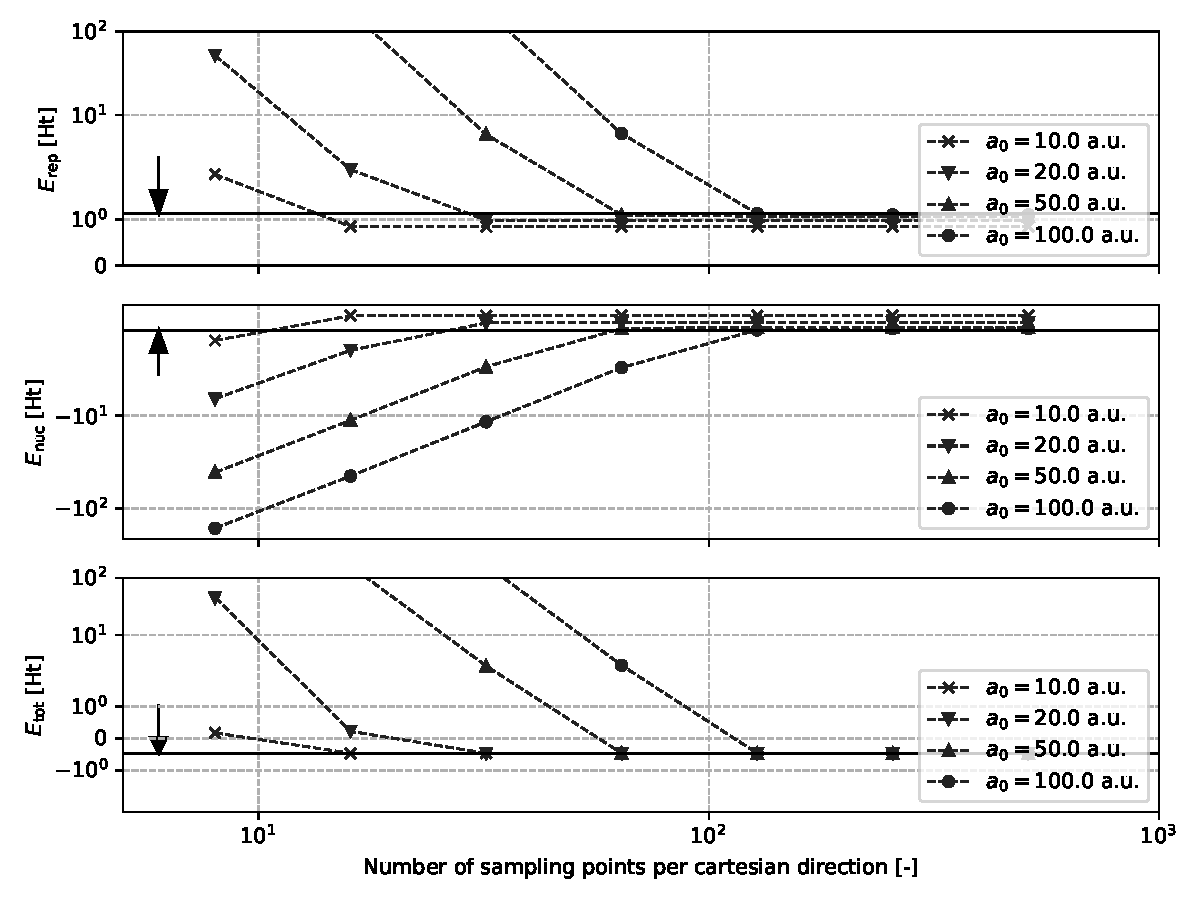
\includegraphics[width=\linewidth]{img/hartree.pdf}
    \captionof{figure}{(top) Electron-electron repulsion and (middle) nuclear attraction energy as function of the number of sampling points per Cartesian direction for various unit cell sizes. The sum of these two terms is plotted in the lower graph. The analytical results are indicated by the dotted lines.}
    \label{fig:electrostatics}
\end{Figure}

For the nuclear attraction energy $E_{\text{nuc}}$, there also exists an analytical solution, which corresponds to

\begin{equation}
    E_{\text{nuc}} = \left<\phi(\vec{r})\left|\frac{1}{r}\right|\phi(\vec{r})\right> = -2\sqrt{\frac{2}{\pi}}.
\end{equation}

In the middle graph in \cref{fig:electrostatics}, the numerical approximation of this value as function of unit cell size and number of plane waves is shown. Again, a relatively poor convergence can be found, especially for the the smallest unit cell ($a_{0} = 10$ a.u.).

Let us now \textbf{combine} $E_{\text{nuc}}$ and $E_{\text{rep}}$ and explore its sum, whose analytical solution is given by

\begin{equation}
    E_{\text{tot}} = E_{\text{nuc}} + E_{\text{rep}} = \frac{2 \left( 1 - \sqrt{2} \right)}{\sqrt{\pi}}
\end{equation}

as function of unit cell size and number of plane waves. The result of this analysis is shown in the bottom graph in \cref{fig:electrostatics}. In contrast to the earlier situation where relatively poor convergence towards the analytical value was observed, here we see that a mere 16 sampling points per Cartesian direction is already sufficient to approximate the analytical solution.
Note that in the toy problem discussed above, we only needed to consider the combination of $E_{\text{nuc}}$ and $E_{\text{rep}}$. For an actual plane-wave density functional theory calculation, one would also need to include the repulsion between the nuclei, correspond to an Ewald sum as discussed in \cref{chap:ewald}.

%
%
%
\subsection{The exchange-correlation potential}

The fundamental idea behind the Kohn-Sham procedure is that the electronic structure of a system of interacting electrons can be approximated by a fictitious system of non-interacting electrons with the same electron density as the interacting one.\cite{1965:kohn} When electrons are non-interacting, the ground state wave function can be found by solving a system of one-electron equations wherein each electron acts under the influence of an effective field $\nu_{\text{eff}}$. The kinetic energy of this system of non-interacting electrons differs from the kinetic energy of interacting electrons. To resolve this, the clever idea of Kohn and Sham was to extract the part that corresponds to the interaction from the kinetic energy as well as any non-classical terms of the electron-electron interaction and put these together in the exchange-correlation term. If we want to make this theory work, an explicit form for $E_{\textrm{xc}}[\rho(\vec{r})]$ is needed.

The most simple exchange-correlation functional corresponds to the local density approximation (LDA), wherein it is assumed that the variations in the electron density are sufficiently small such that the exchange and correlation contributions to the energy $E_{x}$ and $E_{c}$ can be directly derived from the solutions known for the uniform homogeneous electron gas. The exchange-correlation functional thus only depends on the \textbf{local} value of the electron density $\rho(\vec{r})$. The exchange energy for a uniform electron gas is

\begin{equation}
E_{x}[\rho(\vec{r})] = -\frac{3}{4}\left(\frac{3}{\pi}\right)^{1/3} \int d\vec{r}\; \rho^{4/3}(\vec{r}).
\label{eq:chap04:slater_exchange}
\end{equation}

For the self-consistent field procedure, also the functional derivative $\nu_{x}(\vec{r})$ of $E_{x}[\rho(\vec{r})]$ is needed which is given by

\begin{equation}
\nu_{x}(\vec{r}) = -\frac{\delta E_{x}[\rho(\vec{r})]}{\delta \rho(\vec{r})} = \left(\frac{3}{\pi}\right)^{1/3} \rho^{1/3}(\vec{r}).
\end{equation}

Much work is done into formulating a functional for the correlation energy and the most modern density functional theory codes use the implementation of Vosko, Wilk and Nusair. In this implementation, a Padé-approximant interpolation is conducted on accurate numerical calculations using quantum Monte-Carlo of Ceperley and Alder which yields the following recipe to calculate the correlation energy\footnote{From the correlation energy, one can also calculate the correlation potential by means of determining the functional derivative. This is not explicitly shown in this work as the equation is fairly lengthy, yet the function is provided in the source code of PyPWDFT.} as function of the electron density.\cite{1980:vosko,1980:ceperley}

\begin{equation}
E_{c}[\rho] = \frac{A}{2} \left\{ \ln \left( \frac{x^{2}}{X(x)} \right) + \frac{2b}{Q} \tan^{-1} \left( \frac{Q}{2x+b} \right) -\frac{bx_{0}}{X(x_{0})} Y \right\}
\label{eq:vwn5}
\end{equation}

wherein

\begin{equation}
    Y = \left[ \ln \left( \frac{(x-x_{0})^{2}}{X(x)} \right) + \frac{2(b+2x_{0})}{Q} \tan^{-1} \left( \frac{Q}{2x+b} \right) \right]
\end{equation}

and

\begin{align}
	x &= r_{s}^{1/2} \\
	X(x) &= x^{2} + bx + c \\
	Q &= \left(4c - b^{2}\right)^{1/2}.
\end{align}

Herein, $r_{s}$ is the effective electron volume which can be calculated from the density $\rho$ using

\begin{equation}
	r_{s} = \left( \dfrac{3}{4 \pi \rho} \right)^{1/3}.
\end{equation}

The constants for the paramagnetic case, i.e. a spin-unpolarized electron density, are given by $A = 0.0621814$, $x_{0} = -0.409286$, $b = 13.0720$, $c = 42.7198$.

Following the above numerical recipe, one is able to assign an exchange-correlation energy to an arbitrary electron density and furthermore use the corresponding exchange-correlation potential to optimize the Kohn-Sham states. It should however be emphasized once more that the LDA is the most simple form of an exchange-correlation functional and there exist many more functionals with increasing computational complexity and accuracy. However, within the scope of this work I only discuss and use the LDA.